% Created 2021-09-27 Mon 12:03
% Intended LaTeX compiler: xelatex
\documentclass[letterpaper]{article}
\usepackage{graphicx}
\usepackage{grffile}
\usepackage{longtable}
\usepackage{wrapfig}
\usepackage{rotating}
\usepackage[normalem]{ulem}
\usepackage{amsmath}
\usepackage{textcomp}
\usepackage{amssymb}
\usepackage{capt-of}
\usepackage{hyperref}
\setlength{\parindent}{0pt}
\usepackage[margin=1in]{geometry}
\usepackage{fontspec}
\usepackage{svg}
\usepackage{cancel}
\usepackage{indentfirst}
\setmainfont[ItalicFont = LiberationSans-Italic, BoldFont = LiberationSans-Bold, BoldItalicFont = LiberationSans-BoldItalic]{LiberationSans}
\newfontfamily\NHLight[ItalicFont = LiberationSansNarrow-Italic, BoldFont       = LiberationSansNarrow-Bold, BoldItalicFont = LiberationSansNarrow-BoldItalic]{LiberationSansNarrow}
\newcommand\textrmlf[1]{{\NHLight#1}}
\newcommand\textitlf[1]{{\NHLight\itshape#1}}
\let\textbflf\textrm
\newcommand\textulf[1]{{\NHLight\bfseries#1}}
\newcommand\textuitlf[1]{{\NHLight\bfseries\itshape#1}}
\usepackage{fancyhdr}
\pagestyle{fancy}
\usepackage{titlesec}
\usepackage{titling}
\makeatletter
\lhead{\textbf{\@title}}
\makeatother
\rhead{\textrmlf{Compiled} \today}
\lfoot{\theauthor\ \textbullet \ \textbf{2021-2022}}
\cfoot{}
\rfoot{\textrmlf{Page} \thepage}
\renewcommand{\tableofcontents}{}
\titleformat{\section} {\Large} {\textrmlf{\thesection} {|}} {0.3em} {\textbf}
\titleformat{\subsection} {\large} {\textrmlf{\thesubsection} {|}} {0.2em} {\textbf}
\titleformat{\subsubsection} {\large} {\textrmlf{\thesubsubsection} {|}} {0.1em} {\textbf}
\setlength{\parskip}{0.45em}
\renewcommand\maketitle{}
\author{exr0n}
\date{\today}
\title{Calc easy 4}
\hypersetup{
 pdfauthor={exr0n},
 pdftitle={Calc easy 4},
 pdfkeywords={},
 pdfsubject={},
 pdfcreator={Emacs 28.0.50 (Org mode 9.4.4)}, 
 pdflang={English}}
\begin{document}

\tableofcontents



\section{Problems on slide 38}
\label{sec:org55f547a}
\subsection{Problem 36}
\label{sec:orge443271}
$\backslash$[
\begin{aligned}
\lim_{x\to 0}\sqrt{x^3+x^2} sin\frac{\pi}{x}=0
\\& -1 \le sin\frac{\pi}{x} \le 1 \\&\therefore -\left| x \sqrt{x+1} \right| \le x \sqrt{x+1} sin \frac{\pi}{x}\lt \left| x \sqrt{x+1}\right|
\end{aligned}
$\backslash$] \begin{center}
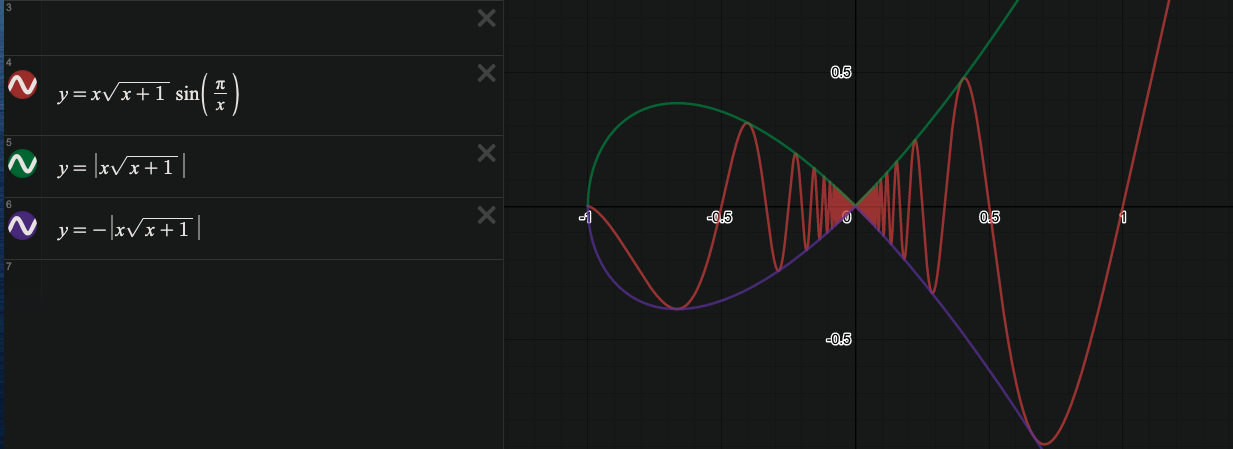
\includegraphics[width=.9\linewidth]{./Pastedimage20200923221014.png}
\end{center} $\backslash$[
\begin{aligned}
\lim_{x\to 0} -\left|x\sqrt{x+1}\right| = -\left|0\sqrt{1}\right| = 0\\
\lim_{x\to 0} \left|x\sqrt{x+1}\right| = -\left|0\sqrt{1}\right| = 0\\
\therefore \lim_{x\to 0} = \sqrt{x^3+x^2}\sin\frac{\pi}{x} = \boxed{0}
\end{aligned}
$\backslash$]

\subsection{Problem 37}
\label{sec:org8e04585}
$\backslash$[
\begin{aligned}
\lim_{x\to 4}4x-9 = 4(4)-9 = 16-9 = 7\\
\lim_{x\to 4}x^2-4x+7 = 4^2 - 4(4) + 7 = 7\\
4x-9 \le f(x) \le x^2 - 4x+7\\
\therefore \lim_{x\to 4}f(x) = \boxed{7}
\end{aligned}
$\backslash$]

\subsection{Problem 38}
\label{sec:org14db517}
$\backslash$[
\begin{aligned}
\lim_{x\to 1}2x = 2(1) = 2\\
\lim_{x\to 1}x^4-x^2+2 = 1 - 1 + 2 = 2\\
2x \le g(x) \le x^2 - x^2 + 2\\
\therefore \lim_{x\to 1}g(x) = \boxed{2}
\end{aligned}
$\backslash$]

\subsection{Problem 39}
\label{sec:org9488553}
This one is doable by just saying that
\(\lim\limits_{x\to 0}x^4cos\frac{2}{x} = \lim\limits_{x\to 0} x^4 \lim\limits_{x\to 0}cos\frac{2}{x} = 0\left(\lim\limits_{x\to 0} cos\frac{2}{x}\right) = 0\).

But we can also do it properly: $\backslash$[
\begin{aligned}
-1 \le cos\frac{2}{x}\le 1\\
\therefore -x^4 \le x^4 cos\frac{2}{x} \le x^4\\
\lim_{x\to 0} -x^4 = 0 = \lim_{x\to 0} x^4 \\
\therefore \lim_{x\to 0}x^4cos\frac{2}{x} = \boxed{0}
\end{aligned}
$\backslash$]

\subsection{Problem 40}
\label{sec:org3f2488b}
\begin{itemize}
\item inspired by
\href{https://github.com/perfectblue/ctf-writeups/tree/master/2020/csaw-quals-2020/take-it-easy}{GUESS
GOD}
\end{itemize}

So originally you notice that \(\sqrt{0}\) is just \(0\) so the thing is
going to be zero in the end either way

But we can guess god our way to the nice functions using this graph

\begin{center}
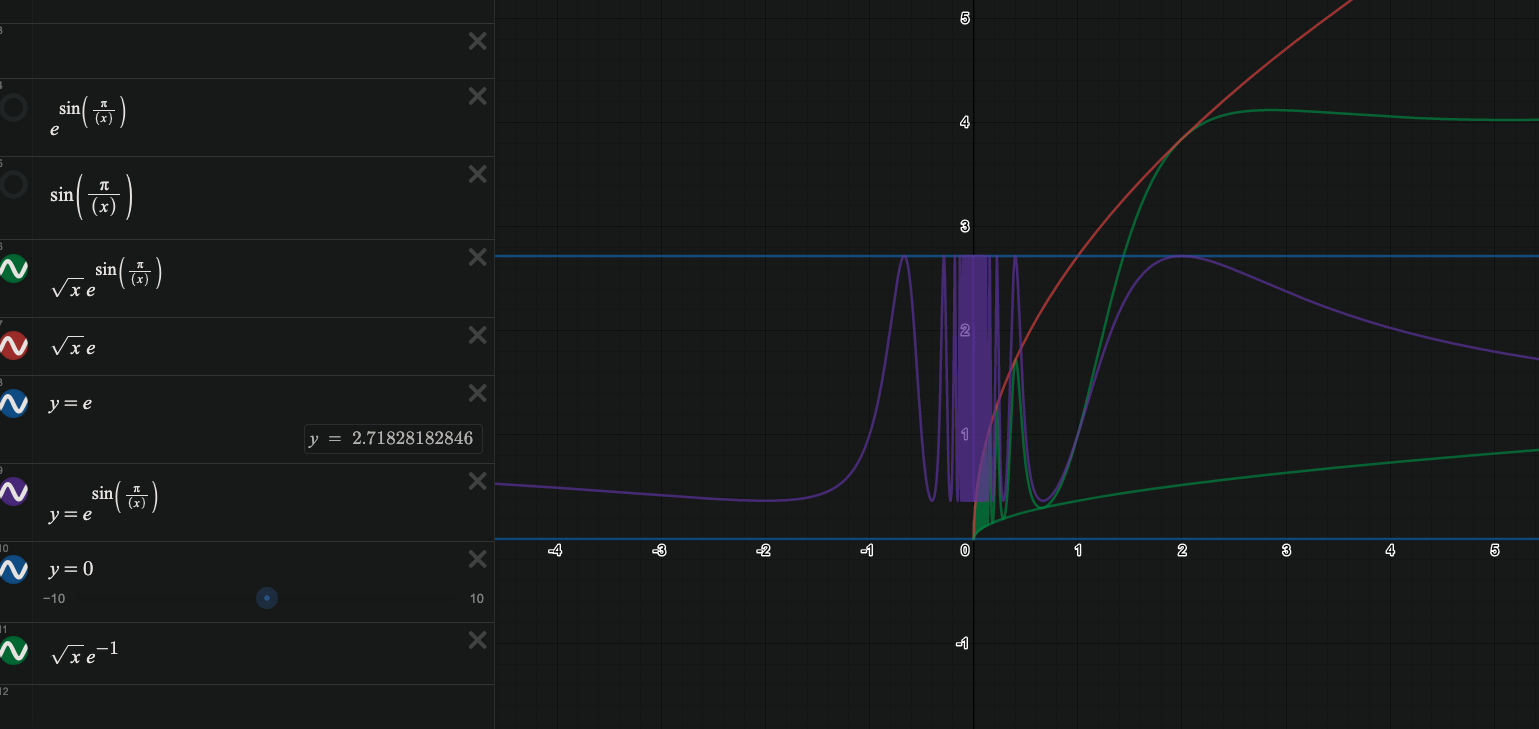
\includegraphics[width=.9\linewidth]{./Pastedimage20200923222859.png}
\end{center}

So we know from earlier that \(-1 \le sin\frac{\pi}{x} \le 1\) and like
taking a psotivie numebr to a power is not gonn make it negative so like
\(e^{sin\frac{\pi}{x}}\) is gonna be more den \(0\)

oh and also because the sin power thingjust makes it fluctuate - we can
prolly ignore that entire term and just try \(\sqrt{x}\)

except sike it's too low it needs to be bigger

\begin{itemize}
\item maybe just multpily by \(e\) liek \(\sqrt{x}e\)
\end{itemize}

great so now we have an upper bound and the lower bound is zero so that
works except maybe we can make a :sunglasses:-er one? - guess god strats
maybe it's the lower bound of the \(\sin{\frac{\pi}{x}}\) exponent so
like \(\sqrt{x}e^{-1}\) and yup thats' work guess god strat always wins

Here's the actual "writeup" $\backslash$[
\begin{aligned}
-1 \le sin{\frac{\pi}{x}} \le 1\\
\therefore& e^{-1} \le e^{sin{\frac{\pi}{x}}} \le e^1\\
\therefore& \sqrt{x}e^{-1} \le \sqrt{x}e^{sin\frac{\pi}{x}} \le \sqrt{x} e\\
\lim_{x\to 0^+} \sqrt{x}e^{-1} = \sqrt{0}e^{-1} = 0\\
\lim_{x\to 0^+} \sqrt{x}e = \sqrt{0}e = 0\\
\therefore& \lim_{x\to 0^+}\sqrt{x}e^{sin\frac{\pi}{x}} = \boxed{0}
\end{aligned}
$\backslash$] thanks for coming to my ted talk

\noindent\rule{\textwidth}{0.5pt}
\end{document}
